
\begin{document}
\pagestyle{fancy}
\fancyfoot{}
\fancyfoot[LO,RE]{\thepage}
\begin{figure}
    
\includegraphics[width=1\linewidth]{Снимок экрана 2023-11-23 в 20.34.57.png}
\end{figure}
\begin{flushright}
    \Large{\textsc{\textbf{Р. П. Шейнцвит}}}
\end{flushright}

\begin{multicols}{2}
Рассмотрим задачу:

\textit{На складе имеются предметы (каждый по одному), вес и стоимость которых указаны в таблице.}
\\

\noindent
\begin{tabular}{c|c|c}
    \hline
    Порядковый&Вес в цент-&Стоимость\\
    номер&нерах&(в рублях)\\
    \hline
    1&11&120\\
    2&7&140\\
    3&6&60\\
    4&5&80\\
    5&12&160\\
    6&9&110\\
    \hline
    Всего:&50&670
\end{tabular}
\\

\textit{Грузоподъемность автомашины — 3200 кг. Требуется так загрузить автомашину, чтобы общая стоимость взятых предметов была как можно большей.}

Очевидно, выгоднее брать предметы, имеющие при малом весе большую стоимость.

Введем понятие \textit{удельной стоимости} предмета $d_i$, то есть стоимости одного центнера $і$-го предмета в рублях: $d_1=10,9; d_2=20; d_3=10; d_4=16; d_5=13,3; d_6=12,2$.

Если загрузить автомашину предметами с наибольшей удельной стоимостью - вторым, четвертым, пятым
и шестым, — то сумма их весов окажется больше грузоподъемности автомашины $(7+15+12+9>32)$.

Если же взять только 2-й, 4-й и 5-й предметы, то машина окажется недогруженной на 8 \textit{ц}. Можно тогда погрузить еще только один 3-й предмет, причем суммарная стоимость получится равной 440 руб., а машина будет недогружена на 2 \textit{ц}. Можем ли мы быть уверены, что не существует лучшего способа загрузки машины?

Может быть, выгоднее оставить какой-либо из предметов с большей удельной стоимостью, но зато уве- личить общую стоимость путем пол- ного использования грузоподъемно-
сти машины?

Как видим, «в лоб» задачу решить трудно. А в реальных условиях, когда речь зачастую идет не о шести, а о шестидесяти предметах, и браться за нее нельзя, не вооружившись математическими методами. Переведем задачу на язык математики (как говорят, математизируем ситуацию).

Пусть $x_i=1$, если $i$-й предмет погружается на автомашину, и $x_i=0$ в противном случае $(i=1\dots6)$. Тогда общая стоимость погруженных предметов равна $120x_1+140x_2+60x_3+80x_4+160x_5+110x_6$, а их общий вес в центнерах равен $11x_1+7x_2+6x_3+5x_4+12x_5+9x_6$.
\newpage
С помощью известных формул геометрии и тригонометрии из теоремы косинусов можно вывести некоторые соотношения, связывающие элементы любого треугольника.

П р и м е р 2. \textit{Доказать, что стороны, углы и площадь S треугольника ABC удовлетворяют соотношению} \[\ctg A+\ctg B+\ctg C=\frac{a^2+b^2+c^2}{4S}.\]

Р е ш е н и е. Из формулы $S=\frac{1}{2}bc\sin A$ находим, что $bc=\frac{2S}{\sin A}.$ Подставив формулу $a^2=b^2+c^2-2bc\cos A$ вместо $2bc$ выражение $\frac{4S}{\sin A}$, получим, соотношение \begin{equation}
    a^2=b^2+c^2-4S\ctg A.
\end{equation}
Следовательно, \[\ctg A=\frac{b^2+c^2-a^2}{4S}\]

П р и м е р 3. \textit{Доказать, что для любого треугольника справедливы неравенства}
\[a) \sin \frac{A}{2}\leq\frac{a}{2\sqrt{bc}}\]\[b) \tg\frac{A}{2}\leq\frac{a}{2h_a},\]
где \textit{a, b, c - стороны треугольника ABC и $h_a$ - высота, проведённая из вершины A.}
\end{multicols}

\newpage
\resizebox{7cm}{!}{
    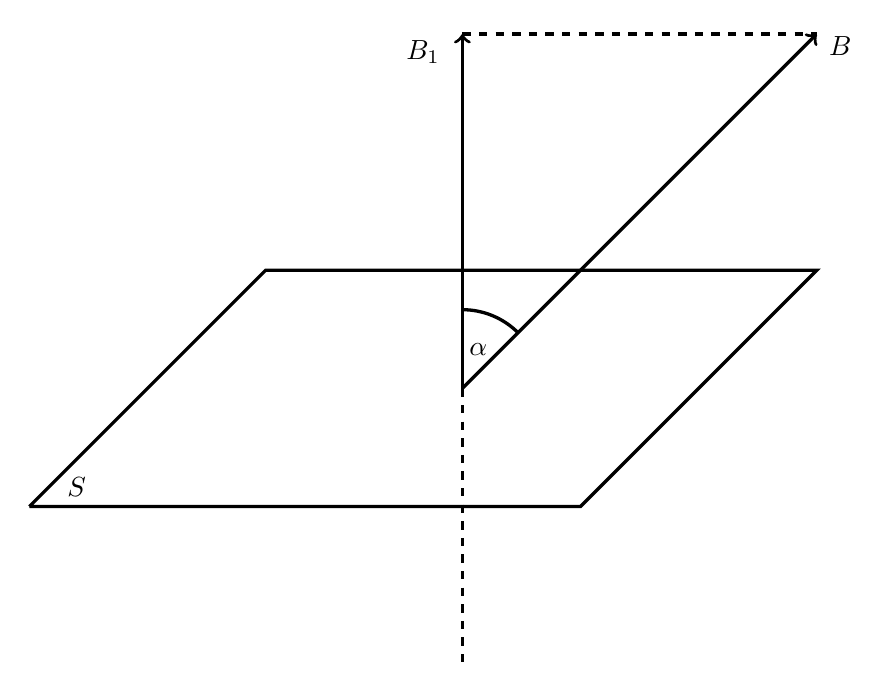
\begin{tikzpicture}
    \draw[very thick] (0,-6) -- (3,-3) -- (10,-3) -- (7,-6) -- (0,-6);
    \draw (0.6,-6) node[above] {$S$};
    \draw[dashed, very thick] (5.5,-4.5) -- (5.5,-8);
    \draw[very thick, ->] (5.5,-4.5) -- (5.5, 0);
    \draw[very thick, ->] (5.5,-4.5) -- (10,0);
    \draw[very thick, dashed] (5.5,0) -- (10,0);
    \draw (5,-0.5) node[above] {$B_1$};
    \draw (10.3,-0.4) node[above] {$B$};
    \draw[very thick] (5.5,-3.5) arc (90:45:1);
    \draw (5.7,-4.2) node[above] {$\alpha$};
    \end{tikzpicture}
}

\textbf{Рис. 1.}
\end{document}